%%%%%%%%%%%%%%%%%%%%%%%%%%%%%%%%%%%%%%%%%
% Short Sectioned Assignment LaTeX Template Version 1.0 (5/5/12)
% This template has been downloaded from: http://www.LaTeXTemplates.com
% Original author:  Frits Wenneker (http://www.howtotex.com)
% License: CC BY-NC-SA 3.0 (http://creativecommons.org/licenses/by-nc-sa/3.0/)
%%%%%%%%%%%%%%%%%%%%%%%%%%%%%%%%%%%%%%%%%

%----------------------------------------------------------------------------------------
%	PACKAGES AND OTHER DOCUMENT CONFIGURATIONS
%----------------------------------------------------------------------------------------

\documentclass[paper=a4, fontsize=11pt]{scrartcl} % A4 paper and 11pt font size

% ---- Entrada y salida de texto -----

\usepackage[T1]{fontenc} % Use 8-bit encoding that has 256 glyphs
\usepackage[utf8]{inputenc}
%\usepackage{fourier} % Use the Adobe Utopia font for the document - comment this line to return to the LaTeX default

% ---- Idioma --------
\usepackage[spanish]{babel}
%\usepackage[spanish]{babel} % Selecciona el español para palabras introducidas automáticamente, p.ej. "septiembre" en la fecha y especifica que se use la palabra Tabla en vez de Cuadro

% ---- Otros paquetes ----

\usepackage{url} % ,href} %para incluir URLs e hipervínculos dentro del texto (aunque hay que instalar href)
\usepackage{amsmath,amsfonts,amsthm} % Math packages
%\usepackage{graphics,graphicx, floatrow} %para incluir imágenes y notas en las imágenes
\usepackage{graphics,graphicx, float} %para incluir imágenes y colocarlas

% Para hacer tablas comlejas
%\usepackage{multirow}
%\usepackage{threeparttable}

%\usepackage{sectsty} % Allows customizing section commands
%\allsectionsfont{\centering \normalfont\scshape} % Make all sections centered, the default font and small caps

\usepackage{fancyhdr} % Custom headers and footers
\pagestyle{fancyplain} % Makes all pages in the document conform to the custom headers and footers
\fancyhead{} % No page header - if you want one, create it in the same way as the footers below
\fancyfoot[L]{} % Empty left footer
\fancyfoot[C]{} % Empty center footer
\fancyfoot[R]{\thepage} % Page numbering for right footer
\renewcommand{\headrulewidth}{0pt} % Remove header underlines
\renewcommand{\footrulewidth}{0pt} % Remove footer underlines
\setlength{\headheight}{13.6pt} % Customize the height of the header

\numberwithin{equation}{section} % Number equations within sections (i.e. 1.1, 1.2, 2.1, 2.2 instead of 1, 2, 3, 4)
\numberwithin{figure}{section} % Number figures within sections (i.e. 1.1, 1.2, 2.1, 2.2 instead of 1, 2, 3, 4)
\numberwithin{table}{section} % Number tables within sections (i.e. 1.1, 1.2, 2.1, 2.2 instead of 1, 2, 3, 4)

\setlength\parindent{0pt} % Removes all indentation from paragraphs - comment this line for an assignment with lots of text

\newcommand{\horrule}[1]{\rule{\linewidth}{#1}} % Create horizontal rule command with 1 argument of height

\graphicspath{ {./images/} }
\usepackage{subcaption}
\usepackage{hyperref}
\usepackage{soul}


%----------------------------------------------------------------------------------------
%	TÍTULO Y DATOS DEL ALUMNO
%----------------------------------------------------------------------------------------

\title{	
\normalfont \normalsize 
\textsc{\textbf{Introducción a la Ciencia de Datos (2019)} \\ Máster Oficial Universitario en Ciencia de Datos e Ingeniería de Computadores \\ Universidad de Granada} \\ [25pt] % Your university, school and/or department name(s)
\horrule{0.5pt} \\[0.4cm] % Thin top horizontal rule
\huge Trabajo Integrador: EDA, Clasificación y Regresión \\ % The assignment title
\horrule{2pt} \\[0.5cm] % Thick bottom horizontal rule
}

\author{Luis Balderas Ruiz \\ \texttt{luisbalderas@correo.ugr.es}} 
 % Nombre y apellidos 


\date{\normalsize\today} % Incluye la fecha actual

%----------------------------------------------------------------------------------------
% DOCUMENTO
%----------------------------------------------------------------------------------------

\begin{document}

\maketitle % Muestra el Título

\newpage %inserta un salto de página

\tableofcontents % para generar el índice de contenidos

\listoffigures

\listoftables

\newpage

%
%\begin{figure}[H] %con el [H] le obligamos a situar aquí la figura
%	\centering
%	\includegraphics[scale=0.6]{e1.png}  %el parámetro scale permite agrandar o achicar la imagen. En el nombre de archivo puede especificar directorios
%	\caption{Progresión de la imagen de E en cada iteración} 
%	\label{fig:e1}
%\end{figure}


%----------------------------------------------------------------------------------------
%	Introducción
%----------------------------------------------------------------------------------------

\section{Introducción}


El presente documento contiene los resultados obtenidos en el Trabajo Teórico/Práctico Integrador para la evaluación de la asignatura Introducción a la Ciencia de Datos. El trabajo está formado por tres apartados, a saber, análisis de datos (en adelante EDA), regresión y clasificación, centrado en dos conjuntos de datos: Wankara para regresión y Vowel para clasificación. Ambos dos forman parte del repositorio de Keel (\cite{keel}), el primero en \cite{wankara} y el segundo en \cite{vowel}. A continuación, describo la estructura del documento. En la primera sección, se desarrolla el análisis exploratorio de ambos datasets. A continuación, tras sacar las conclusiones correspondientes, ataco el problema de regresión y, por último, el de clasificación.






%----------------------------------------------------------------------------------------
%	Análisis de datos
%----------------------------------------------------------------------------------------

\section{Análisis exploratorio de datos (EDA)}

\subsection{Conjunto de datos Wankara}

\subsection{Conjunto de datos Vowel}

El presente conjunto de datos contiene información sobre el reconocimiento de las once vocales existentes en inglés por parte de 15 interlocutores independientes. Es un problema de clasificación de once clases (las once vocales inglesas) con trece características, diez de ellas reales y tres enteras. A pesar de ser numéricas, esas tres variables son realmente categóricas, dado que

\begin{itemize}
	\item TT (0/1): Indica si la instancia es de entrenamiento (0) o test (1).
	\item Sex (0/1): Indica el género del hablante en dicha instancia.
	\item SpeakerNumber [0,14]: Indica el interlocutor de la instancia.
\end{itemize}

\begin{figure}[H] %con el [H] le obligamos a situar aquí la figura
	\centering
	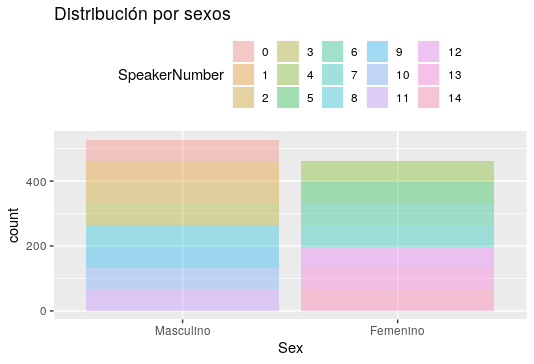
\includegraphics[scale=0.6]{dist-sexos.png}  %el parámetro scale permite agrandar o chicar la imagen. En el nombre de archivo puede especificar directorios
	\caption{Distribución por sexos de los interlocutores} 
	\label{fig:dist-sex}
\end{figure}

Por tanto, esas variables se pueden interpretar como factores más que numéricas. De hecho, TT será ignorada en el EDA porque es conveniente realizar el estudio sobre los datos al completo. Por tanto, tras estas modificaciones contamos con diez variables reales (F0-F9), dos factores (sexo y número de interlocutor) y once clases (0-10), con un total de 990 instancias. 

Para explorar los datos, en primer lugar, calculo un resumen estadístico de cada variable y su dispersión. En las variables categóricas encontramos:

\begin{itemize}
	\item Cada interlocutor tiene 66 apariciones en el conjunto de datos.
	\item 528 de ellos son hombres y 462 mujeres.
\end{itemize}

Para las variables numéricas, los resultados son los siguientes:

\begin{table}[H]
	\resizebox{\textwidth}{!}{\begin{tabular}{|c|c|c|c|c|c|c|c|c|c|c|}
		\hline
		& \textbf{F0} & \textbf{F1} & \textbf{F2} & \textbf{F3} & \textbf{F4} & \textbf{F5} & \textbf{F6} & \textbf{F7} & \textbf{F8} & \textbf{F9} \\ \hline
		\textbf{Min}     & -5.211      & -1.274      & -2.487      & -1.409      & -2.127      & -0.836      & -1.537      & -1.293      & -1.631      & -1.68       \\ \hline
		\textbf{1st Qua} & -3.888      & 1.052       & -0.97575    & -0.0655     & -0.769      & 0.196       & -0.307      & -0.09575    & -0.704      & -0.548      \\ \hline
		\textbf{Mediana} & -3.146      & 1877        & -0.5725     & 0.4335      & -0.299      & 0.552       & 0.022       & 0.328       & -0.3025     & -0.1565     \\ \hline
		\textbf{Media}   & -3.204      & 1.882       & -0.50777    & 0.5155      & -0.3057     & 0.6302      & -0.004365   & 0.33655     & -0.30298    & -0.07134    \\ \hline
		\textbf{3th Qua} & -2.603      & 2.738       & -0.06875    & 1.096       & 0.1695      & 1.0285      & 0.2965      & 0.77        & 0.09375     & 0.371       \\ \hline
		\textbf{Max}     & -0.941      & 5.074       & 1.431       & 2.377       & 1.831       & 2.327       & 1.403       & 2.039       & 1.309       & 1.396       \\ \hline
		\textbf{SD}      & 0.8689872   & 1.1752720   & 0.7119483   & 0.7592613   & 0.6646023   & 0.6038711   & 0.4619268   & 0.5733020   & 0.5701616   & 0.6039855   \\ \hline
	\end{tabular}}
	\caption{Resumen estadístico y desviación típica de las características reales}
\end{table}

Como se puede observar, el rango y el dominio de cada variable es distinto, lo que podría condicionar el rendimiento de los posteriores algoritmos que utilizaremos. Por tanto, será necesario un reescalado de las mismas para evitar esa discriminación positiva de unas variables respecto a otras sólo por ser "mayores". \\

A continuación, presento las 10 variables numéricas con más detenimiento. Una de las características principales de este conjunto de datos es que, si se estudia como un todo, el comportamiento de las variables a veces puede parecer errático. Sin embargo, no se debe soslayar el hecho de que tenemos una variable categórica, la del sexo, que nos hace prácticamente crear dos conjuntos de datos cuasi-independientes: hombres y mujeres, donde sí que encontramos correlaciones y claves para entender el funcionamiento de las características. Como digo, presento cada una de las variables, primero estudiándola en conjunto y luego separando por sexo. Para comprobar si las variables siguen una distribución normal, se han utilizado el test de Shapiro-Wilk (\cite{10.1093/biomet/52.3-4.591}) y la corrección de Lilliefors del test de Kolmogorov-Smirnov (\cite{10.1080/01621459.1967.10482916}). Además, para estudiar el comportamiento tanto por sexo como por interlocutor, represento vía boxplots cada variable.
\newpage

\subsubsection{F0}

Presentamos la variable F0. En primer lugar, reflejo un resumen estadístico de la misma así como su histograma diferenciando entre hombres y mujeres.
\begin{itemize}
	\item Media: -3.204
	\item Mediana: -3.146
	\item Desviación típica: 0.8689872
	\item Rango: [-5.211,-0.941]
	\item Primer y tercer cuartiles: (-3.888,-2.603)
	\item Asimetría: 0.0662973
	\item Curtosis: -0.4974651
\end{itemize}

\begin{figure}[H] %con el [H] le obligamos a situar aquí la figura
	\centering
	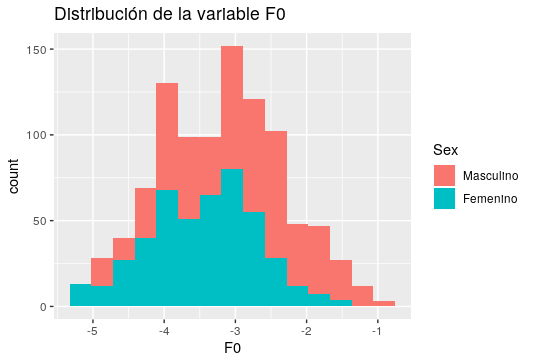
\includegraphics[scale=0.6]{dist-F0.png}  %el parámetro scale permite agrandar o chicar la imagen. En el nombre de archivo puede especificar directorios
	\caption{Histograma de la variable F0} 
	\label{fig:hist-F0}
\end{figure}

Pasamos a comprobar si F0 se distribuye según una normal. Para ello, establecemos los tests de hipótesis de Shapiro-Wilk y Lilliefors (Kolmogorov-Smirnov) con los siguientes resultados:

\begin{figure}[H]
	\centering
	\begin{subfigure}{.5\textwidth}
		\centering
		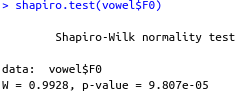
\includegraphics[width=.7\linewidth]{sw-F0.png}
		\caption{Shapiro-Wilk}
		\label{fig:sw-F0}
	\end{subfigure}%
	\begin{subfigure}{.5\textwidth}
		\centering
		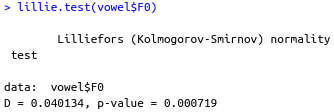
\includegraphics[width=.7\linewidth]{l-F0.png}
		\caption{Lilliefors}
		\label{fig:l-F0}
	\end{subfigure}
	\caption{Tests de normalidad sobre F0}
	\label{fig:normF0}
\end{figure}

Como los p-valores son menores que 0.05, rechazamos la hipótesis nula (la variable sigue una distribución normal). \\


A continuación presento los boxplots:

\begin{figure}[H]
	\centering
	\begin{subfigure}{.5\textwidth}
		\centering
		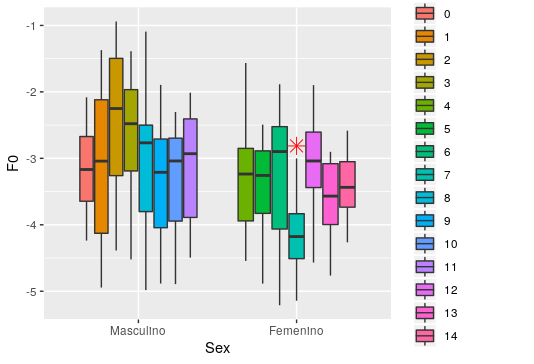
\includegraphics[width=.9\linewidth]{bps0.png}
		\caption{Por sexo}
		\label{fig:bps0}
	\end{subfigure}%
	\begin{subfigure}{.5\textwidth}
		\centering
		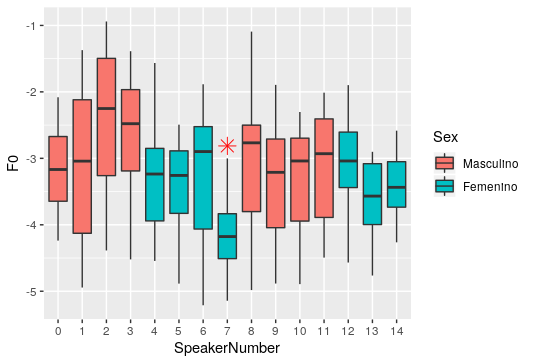
\includegraphics[width=.9\linewidth]{bpsn0.png}
		\caption{Por interlocutor}
		\label{fig:bpsn0}
	\end{subfigure}
	\caption{Boxplot para F0 estudiando sexos e interlocutores}
	\label{fig:bf0}
\end{figure}

Como se puede ver, existe un outlier en el interlocutor 7. Además, observamos que los valores para los hombres tienden a ser mayores que para las mujeres. \\

Si ahora estudiamos los tests de normalidad por sexos, encontramos los siguientes resultados:

\begin{figure}[H]
	\centering
	\begin{subfigure}{.5\textwidth}
		\centering
		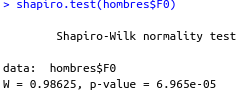
\includegraphics[width=.6\linewidth]{swh-F0.png}
		\caption{Shapiro-Wilk}
		\label{fig:swh-F0}
	\end{subfigure}%
	\begin{subfigure}{.5\textwidth}
		\centering
		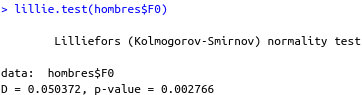
\includegraphics[width=.6\linewidth]{lh-F0.png}
		\caption{Lilliefors}
		\label{fig:lh-F0}
	\end{subfigure}
	\caption{Tests de normalidad sobre F0 (hombres)}
	\label{fig:normhF0}
\end{figure}

En este caso, aunque también se rechaza la hipótesis de normalidad, el test de Lilliefors arroja un resultado menor pero cercano a 0.05, por lo que parece acercarse más la variable en los hombres a una distribución normal que con el conjunto completo. \\

Para las mujeres,

\begin{figure}[H]
	\centering
	\begin{subfigure}{.5\textwidth}
		\centering
		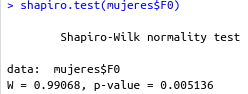
\includegraphics[width=.6\linewidth]{swm-F0.png}
		\caption{Shapiro-Wilk}
		\label{fig:swm-F0}
	\end{subfigure}%
	\begin{subfigure}{.5\textwidth}
		\centering
		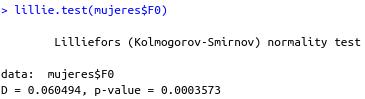
\includegraphics[width=.6\linewidth]{lm-F0.png}
		\caption{Lilliefors}
		\label{fig:lm-F0}
	\end{subfigure}
	\caption{Tests de normalidad sobre F0 (mujeres)}
	\label{fig:normmF0}
\end{figure}

se encuentran unos p-valores menores que para los hombres, por lo que también se rechaza la hipótesis de normalidad.
%----------------------------------------------------------------------------------------
%	Regresión
%----------------------------------------------------------------------------------------

\section{Problema de regresión: Wankara}





%----------------------------------------------------------------------------------------
%	Clasificación
%----------------------------------------------------------------------------------------

\section{Problema de clasificación: Vowel}


\newpage
\section{Bibliografía}

%------------------------------------------------

\bibliography{citas} %archivo citas.bib que contiene las entradas 
\bibliographystyle{plain} % hay varias formas de citar

\end{document}
